%----------------------------------------------------------------------
\section{More on Property Graph Model}
%----------------------------------------------------------------------
We have introduced about property graph model in Introduction part. We know that in property graph model, each node and edge could have arbitary number and type of properties. A type of property is represented by 

NodeType.PropertyType

For instance User.Age represents "Age" property on "User" node.

In order to identify a node or edge, a unique ID is assigned to each node and edge.  In this thesis we represent a type of property by 

ID(node) or ID(edge)

to represent unique ID of a node or edge.

%----------------------------------------------------------------------
\section{Graph OLAP}
%----------------------------------------------------------------------
Three key elements of a graph OLAP are structure, dimension, and measure. Taking Query \#1 as an example: 
 
Question: 	Does high upvotes of a user indicates a high-quality post? 
Query: 		Get average post score grouped by user’s upvotes. 
 
This query is on all the following structures:

\begin {figure}[H]
\centering

\includegraphics[scale=1]{pic/21.png}
\end{figure}

We say that (User)-[User\_owns\_post]->(Post) is the structure of Query \#1.
The query is aggregated by (grouped by) user’s upvotes. We say that {User.Upvotes} is the dimension of Query \#1.
The query is aggregated on avarage of post’s score.  We say that {AVG(Post.Score)} is the meansure of Query \#1. 
 
Similarly, for Query \#2:

Question: 	Similar to Query \#1. But this time we want to take a closer look at Query \#1 for different types of questions. 

Query: 		Get average post score grouped by user’s upvotes and post’s post types. 

Structure:	(User)-[User\_ownspost]-(Post)

Dimensions:	{User.Upvotes, Post.PostTypeId}

Measures:	{AVG(Post.Score)}
 
Notice that Query \#2 adds Post.PostTypeId to Query \#1’s dimensions. That is to say, Query \#2 asks for a more detailed partitions over dimentions. We call Query \#2 a drill-down from Query \#1, and  Query \#1 a roll-up from Query \#2. Such roll-up and drill-down operations allow us to navigate up and down through the dimensional lattice of all possible property combinations. 

\begin {figure}[H]
\centering
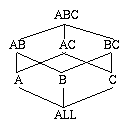
\includegraphics[scale=1]{pic/22.png}
\end{figure}

Query \#3:

Question: 	In year 2017, which is the weighted average age of users? For instance is ‘python’ more trendy than ‘c’ among young users?
 
Query: 		Get average user age grouped by users’ 2017 posts’ tags. 

Structure:	(User)-[User\_owns\_post]-(Post)-[Post\_hastag\_Tag]-(Tag)

Dimensions:	{Tag.Tagname}

Measures:	{AVG(User.Age)}
 
In Query \#3, a requirement that post must be created in year 2017 picks out a particular subset of  all (User)-[User\_owns\_post]-(Post)-[Post\_hastag\_Tag]-(Tag) candidates. In OLAP this is called “slicing” operation. Slicing operation allows users to view the data with filtering requirements on selected properties. 
 
In this thesis we call {Post.Year=2017} a "slicing condition" of Query \#3.
 
To summarize, graph OLAP allows clients to aggregate different structures, over different dimensions, on different measures. Clients can change their views by performing roll-up, drill-down, and slicing freely and interactively.


%----------------------------------------------------------------------
\section{Graph Databases}
%----------------------------------------------------------------------


We have discussed about property graphs and OLAP over property graphs on a high level. This leads us to a question. How are property graphs actually stored and managed in database systems? 
 
There are two major types of databases that store and process graph data: traditional relational databases and graph databases. 
 
Relational databases adopt traditional ways of modeling data in form of entity and relationship tables. For instance, for the following property graph, which consists 1 user and his or her 3 posts. A relational database stores the property graph as 3 tables:

\begin {figure}[H]
\centering
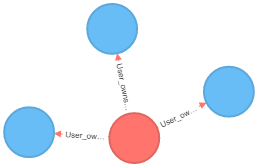
\includegraphics[scale=0.9]{pic/4.png}
\end{figure}

Table-User
\begin{center}
\begin{tabular}{ l | l }  
	Uid	&{All user properties}	\\ \hline 
	1	&{Property values} \\
\end{tabular}
\end {center}

Table-Post
\begin{center}
	\begin{tabular}{ l | l }  
		Pid	& {All post properties}	\\ \hline 
		1	&{Property values} \\
		2	&{Property values} \\
		3	&{Property values} \\
	\end{tabular}
	\end {center}	
 
Table-Owns
\begin{center}
	\begin{tabular}{ l | l }  
		Uid	& Pid	\\ \hline 
		1	&1 \\
		1	&2 \\
		1	&3 \\
	\end{tabular}
	\end {center}

 
There are two drawbacks of storing property graphs in relational databases. First, each node or edge of in property graph could have arbitrary types of properties. However, schemas of relational tables restrict nodes or edges of a same type to have a uniform set of properties (attributes). Second and more importantly, edges are not stored as a separate table. For instance, we cannot directly query all the posts of a given user without joining User and Own tables in the above example.
 
Graph databases solve the above two issues by directly adopting property graph structures to store data. In graph databases, edges are stored not as independant tables but directly attached to related nodes using data structures such as adjacency lists. Many graph database applications have been implemented and commercialized. One of the popular ones is Neo4j.
 
Relational databases and graph databases both have their own strengths in term of query processing. However it is generally accepted that graph databases perform better at property graph data processing as it conforms more with the actual graph structure. 

%----------------------------------------------------------------------
\section{Neo4j}
%----------------------------------------------------------------------
Neo4j is one of the most popular graph databases which holds atomicity, consistency, isolation, durability (ACID). 
 
Instances are modeled and stored as  property graphs in Neo4j. Like other graph databases, edges are not stored as physically separate tables, but directly attached to their nodes. One special thing about Noe4j’s property graph is that its nodes and edges can be labeled with any number of labels (similar to entity and relationship types). For instance a node referring to a student could have various labels such as “student”, “people” etc. 

Cypher is Neo4j’s query language, which is expressive and simple. Here are some examples of Cypher queries:

Aggregation query: For answers(Post.PostTypeId=2), what is the average score group by different user upvotes?
 
match (u:User)-[r:User\_owns\_Post]->(p:Post) where p.PostTypeId="2" return u.Upvotes, AVG(p.Score)
 
Here “User” and “Post” are labels, PostTypeId and Score are properties of “Post” node, “Upvotes” is property of “User” node.
 
Neo4j is written in Java. While applications in various languages could interact the server by issuing queries with its own BOLT protocol(which is binary and more efficient than HTTP).  

\begin {figure}[H]
\centering
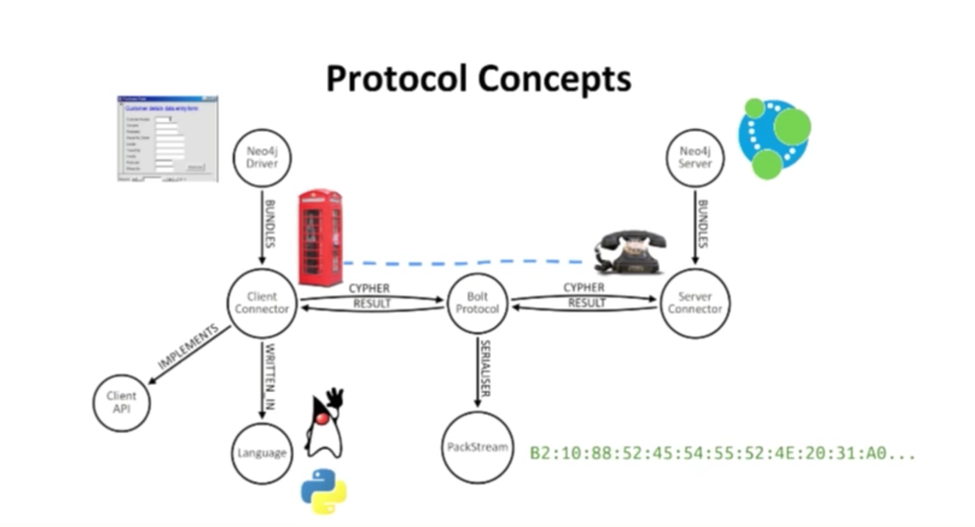
\includegraphics[scale=0.4]{pic/23.png}
\end{figure}


%----------------------------------------------------------------------
\section{Graph Aggregation Paper Summary}
%----------------------------------------------------------------------

Numerous papers have been published on graph aggregation. 

Cube-based [1] proposes the concept of  graphs enriched by cubes. Each node and edge of the considered network are described by a cube. It allows the user to quickly analyze the information summa-
rized into cubes. It works well in slowly changing dimension problem in OLAP analysis.

Gagg [2] introduces an RDF graph aggregation operator that is both expressive and flexible. It provides a formal definition of Gagg on top of SPARQL Algebra and defines its operational semantics and describe an algorithm to answer graph aggregation queries. Gagg achieves significant improvements in performance compared to plain-SPARQL graph aggregation.

Pagrol [3] provides an efficient MapReduce-based parallel graph
cubing algorithm, MRGraph-Cubing, to compute the graph cube
for an attributed graph. 

Graph Cube [4] introduces Graph Cube, a new data warehousing model that supports OLAP queries effectively on large multidimensional networks. It takes account of both attribute aggregation and structure summarization of the networks. In order to deal with “curse of dimensions”, a greedy algorithm framework is introduced for partial materialization of cuboids.

Snapshot [5] studies dimensions and measures in the graph OLAP scenario and furthermore develops a conceptual framework for data cubes on graphs. It differentiates different types of measures(distributive and holistic etc) by their properties during aggregation. It looks into different semantics of OLAP operations, and classifies the framework into two major subcases: informational OLAP and topological OLAP. It points out a graph cube can be fully or partially materialized by calculating a special kind of measure called aggregated graph. 


We summarize some of the most related ones as follows:
 
 \begin{center}
 	\begin{tabular}{ | c | c | c | c | c |  } 
 		\hline 
 		 & Input graph & Query pattern & Layer structure & Highlight\\ \hline Cube-based [1] & property graph & simple relation & yes & cubes on edges and nodes\\ \hline Gagg [2] & property graph & all exact-match patterns & no & structural patterns\\ \hline Pagrol [3] & property graph & edge and node attributes & yes & Map-Reduce distributed computing\\ \hline Graph Cube [4] & homogenous nodes and edges & node attributes & yes & partial materialization algorithm\\ \hline Snapshot [5] & property graph & edge and node attributes & yes & distributive and holistic measures\\ \hline 
 	\end{tabular}
 	\end {center}

 
 
From the summary we can categorize the papers into two kinds: 
 
First, like Graph Cube[4], focuses on a simple subset of property graphs(e.g. graphs with only homogenous nodes and edges) and propose optimizations on OLAP query processing. The optimizations are attribute-aware, and since the nodes and edges are of only one kind queries over different structures and structure-aware optimizations are out of the scope. 
 
Second, like Gagg [2], focus on an abstract high-level framework that process generic queries over generic property graphs. However, query optimizations are not focused.  
 
Therefore it is very meaningful to explore faster structure-aware OLAP processing over general property graphs.



%----------------------------------------------------------------------
\section{Graph Cube}
%----------------------------------------------------------------------

In Graph Cube [4], concepts of graph cube is introduced. Given a particular structure S, a property set P, and measure set M. We can aggregate over S on 2\^{}|P| different combinations of dimensions. These 2\^{}|P| queries can be mapped as a lattice structure, where each combination of dimensions corresponds to a cuboid in the lattice. We call the lattice structure of these 2\^{}|P| queries a graph cube.

\begin {figure}[H]
\centering
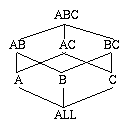
\includegraphics[scale=1]{pic/22.png}
\end{figure}

It has been pointed out that as long as if domain of measure is within \{count, sum, average\} and M contains count(*), the following feature holds:
 
Given any two cuboids C1 and C2 from the same graph cube, as long as dimension(C2) is a subset of dimension(C1), result of C1 can be used to generate result of C2. This is to say once a cuboid is materialized, all roll-up operations from this cuboid could be processed simply by scanning the materialized cuboid result. This will dramatically decrease roll-up operation time compared to aggregation from data graph(often of larger size, disk I/O), scanning materialized cuboid result(often of smaller size) is often much faster.


 
Ideally we can materialize all cuboids. But when number of dimension is large, number of cuboids grows exponentially, making total materialization impossible due to overwhelming space cost. To solve this Graph Cube [4] proposed a partial materialization algorithm on graph cube. It is a greedy algorithm and the score function is based on benefits of deduction of total computation cost.
